\section{Evaluation}
\label{sec:eval}
In this paper, we attempt to answer performance concerns with switching to a switchless topology from either fat-tree or hierarchical set-up: how much slower would running a workload like weather modeling or Hadoop? To this end, we simulate a micro-benchmark with parameters approximate that of real workloads on 2 switchless topologies (mesh and cube), and 2 traditional topologies (fat-tree and hierarchical). As alluded to in Section~\ref{sec:arch}, we do not expect switchless to have higher performance than a fat-tree. Yet, with the massive force of low-cost attached to switchless, we would hope that any performance degradation would not be so drastic.

%We also ran a few more benchmarks such as a bandwidth stress test to see the effect of increasing data transfer rate, as well as the efficiency of UDP vs TCP.
We also ran a few more benchmarks such as the overhead of UDP vs TCP in the data center setting, as well as IP routing version dimension-ordered routing.

\subsection {Methodology}
For performance evaluation, we use ns3, an open-source discrete-event network simulator devleoped by network research community. We modified the significant portion of the simulator for our purpose. These modifications include addition of dimension-ordered routing protocol, addition of various network topologies, etc. ns-3 simulator augmented with our modifications models all five OSI communication layers to the certain detail.

As it is hard to define a small representative application for the data center, we used a micro-benchmark that can be configured to model various different data center application's communication pattern. For example, this micro-benchmark can be configured to generate simple all-to-all style communication traffic with set intensity. On the other hand, it can also be configured to generate sporadic communications between two random nodes. Note that there are many other possible configurations which can model varying communication types.

% benchmark configurations (common)
The default configurations for all simulations are detailed in Table~\ref{tab:configurations}, unless noted specifically.
% # host: 512
% Ethernet links: 1Gbps
% hierarchical: 1 core, balanced fan-outs (agg / edge == edge / host)
% link/switching latency is 500ns for all topologies!!!!!!!!!!! (might be wrong)
% cube z-dimension limit is 40
% all topologies are running on UDP
% switchless are using dimension ordered routing
% 4KB packet length

\subsection {Results}
% Results -- 
% (1) Impact of topology change on performance
% (2) Impact of routing change on performance
% (3) Application Sensitivity (Different application configurations)
% (4) Scalability (host count change)


\subsubsection{N-Body simulation performance}
\newcommand{\nbody}{N-Body}
In a classic \nbody simulation, we have an all-to-all communication pattern. In Figure~\ref{fig:nbody_packetdelay} we have the latency distribution graph of all packets sent in one computation round of an \nbody simulation; in Figure~\ref{fig:nbody_latency} we have the longest packet delay--the global communication latency of a computation round--compared.

\captionsetup[subfloat]{captionskip=-0.003in}
\begin{figure}
    \centering
    \subfloat[Packet delay distribution]
    {
        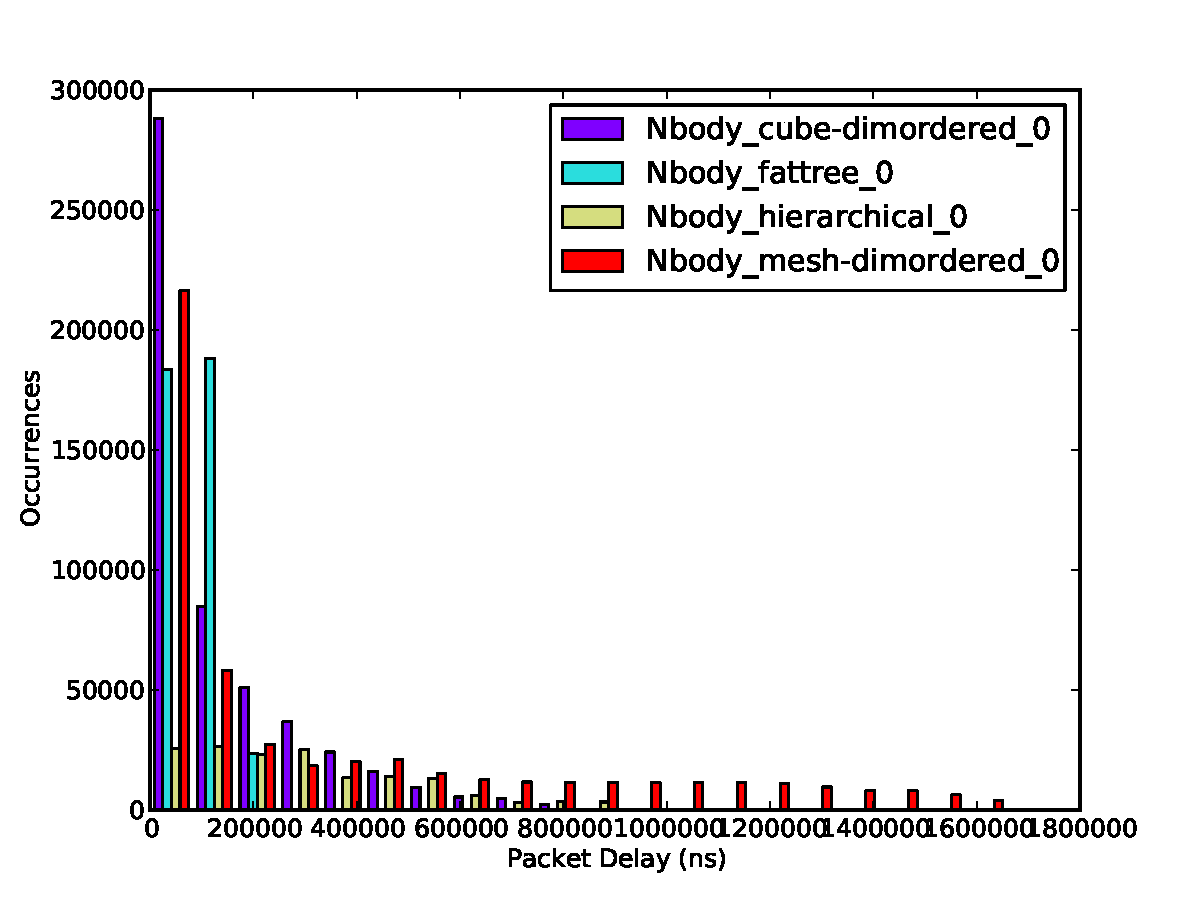
\includegraphics[width=0.4\textwidth]{Nbody_cube-dimordered_parsed_delay.pdf}
        \label{fig:nbody_packetdelay}
    }
    \\
    \vspace{-0.1in}
    \subfloat[Longest delay]
    {
        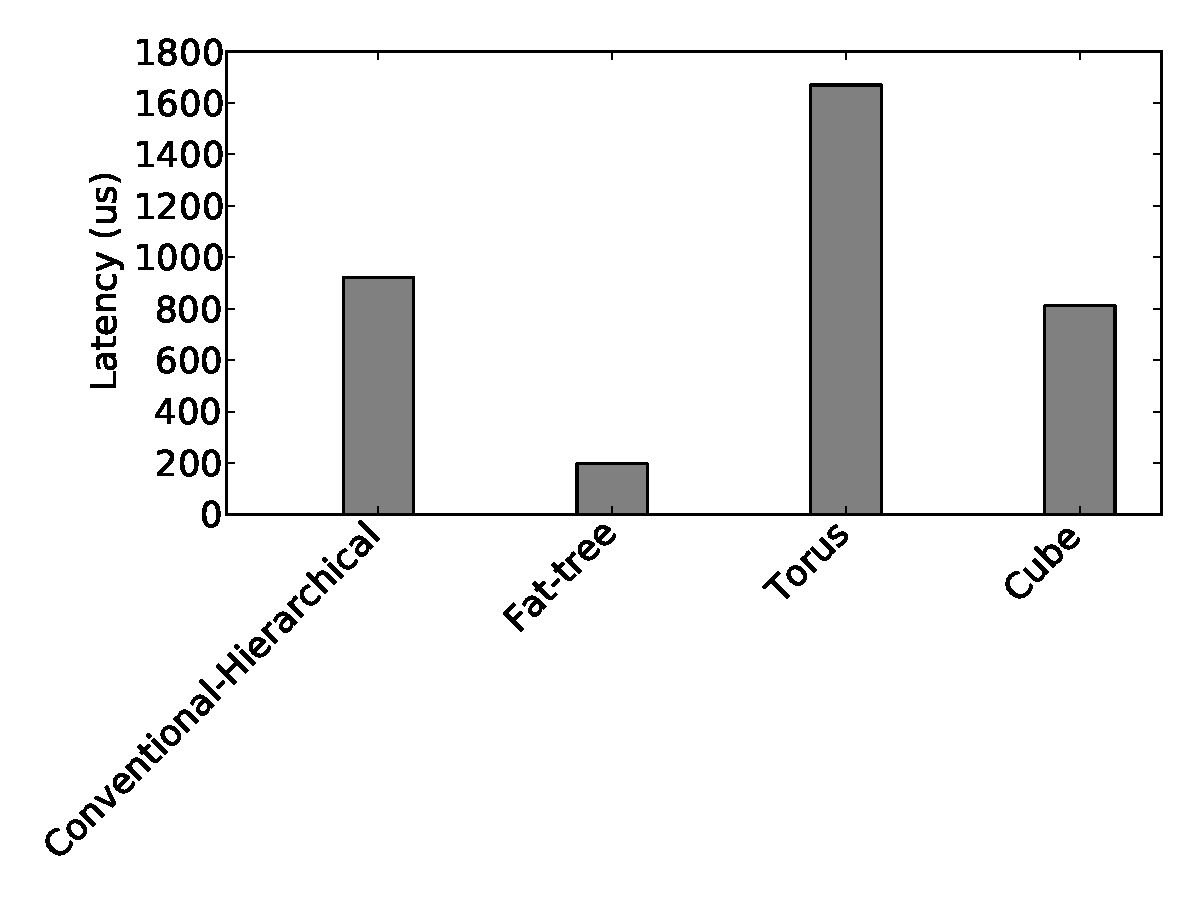
\includegraphics[width=0.4\textwidth]{Nbody_cube-dimordered_parsed_latency.pdf}
        \label{fig:nbody_latency}
    }
    \vspace{-0.07in}
    \caption{N-Body simulation results}
    \label{fig:common_topos}
\end{figure}

First, looking at the packet delay graph, we see that while switchless topologies have higher occurences of really short packet delay (nodes close together), they also have a long tails (nodes far away) that limit the global computation throughput of an \nbody simulation. As shown in Figure~\ref{fig:nbody_latency}, fat-tree is about 4 times faster than cube and hierarchy, and as much as 7 times faster than mesh topology.

On the other hand, it doesn't necessarily mean that simulation under fat-tree is 4 times faster than cube: the computational time is needed to compute overall performance.
% perhaps we need a plot here, comparing different topologies' time in y axis with computational time in the x axis.

\subsubsection{Weather modeling performance}
In weather modeling, we have a lockstep, all-to-neighbors communication; this means that every node in the system communicates to six other nodes representing up, down, north, south, east, and west. This workload should map very well to switchless topologies, whereas hierarchical and fat-tree can still do very well but the energy cost would be significantly more.

\captionsetup[subfloat]{captionskip=-0.003in}
\begin{figure}
    \centering
        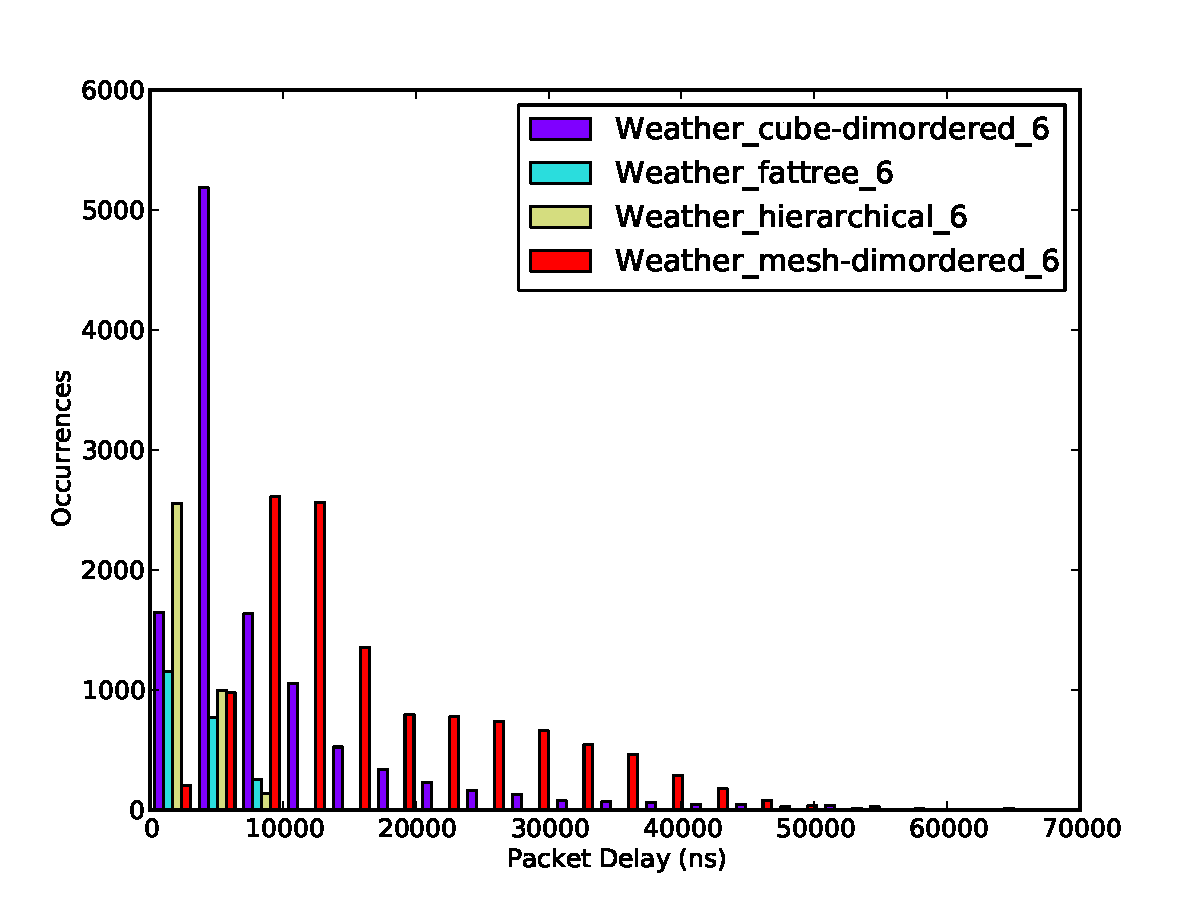
\includegraphics[width=0.4\textwidth]{Weather_cube-dimordered_delay}
        \label{fig:weather_packetdelay}
    \caption{N-Body simulation results}
\end{figure}

Figure~\ref{fig:weather_packetdelay} shows the distribution graph of all packets transferred of a computation round in a weather modeling simulation with 6 neighbors. For a reason not quite understood, a long tail can still be seen with both cube and mesh topology.

On the oher hand, there are a few reasons why hierarchical or fat-tree has good performance. The most conspicuous reason is that our micro-benchmark doesn't map exactly to a weather modeling simulation in that for each node we pick the 6 closest neighbors, which will always be in the same rack. If time allows, we will adjust the parameters for a more accurate results.

\subsubsection{TCP vs UDP}
Data center operators usually run TCP as the level 4 networking stack for better compatibility with MAN and WAN. However, TCP is "heavier" than UDP as a protocol, especially within data centers where packet drops are rare. As we utilize a full networking stack simulator for our study, we implement our topologies with both TCP and UDP and run a simulation exercise to see how the overheads compare.

What we found was that, at least for our simulation set up (as described in Methodology), TCP has about the same performance as UDP, but packet drops are more frequent, leading to completion time timing out

\subsubsection{Dimension-ordered vs IP}
As mentioned, for switchless topologies, we had two implementations: one with TCP/IP routing, and the other one with dimension-ordered routing commonly used in NoC for deadlock avoidance. In our simulation, as shown in Figure~\ref{fig:dimension_ordered}, we found that for some reason dimension-ordered routing is slower than IP. One possible reason for this is that dimension-ordered protocol restricts the possible data paths that packet can traverse through, and so introduces bandwidth contentions that otherwise might not exist in traditional IP routing.

\captionsetup[subfloat]{captionskip=-0.003in}
\begin{figure}
    \centering
        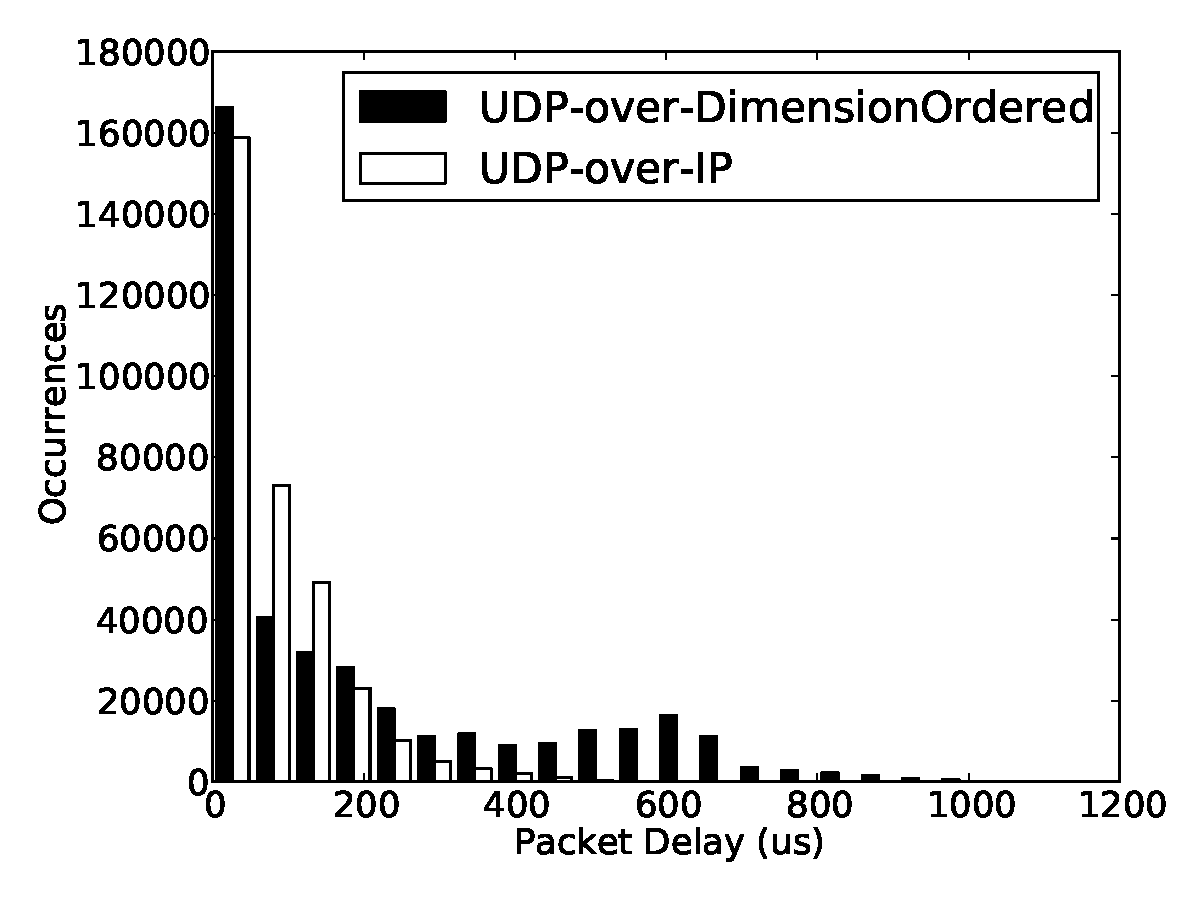
\includegraphics[width=0.4\textwidth]{dimension_ordered_udp}
        \label{fig:dimension_ordered}
    \caption{Packet latency distribution of a mesh network running UDP on top of either IP or dimension-ordered protocol.}
\end{figure}

